\documentclass{sig-alternate}
\usepackage{url}
\sloppy

\begin{document}
\conferenceinfo{ISSTA'06,} {July 17--20, 2006, Portland, Maine, USA.}

\CopyrightYear{2006}

\crdata{1-59593-263-1/06/0007} 


\title{Automated Testing of Stochastic Systems: \\
A Statistically Grounded Approach}

\numberofauthors{3}

% Put no more than the first THREE authors in the \author command
\author{
%
% The command \alignauthor (no curly braces needed) should
% precede each author name, affiliation/snail-mail address and
% e-mail address. Additionally, tag each line of
% affiliation/address with \affaddr, and tag the
%% e-mail address with \email.
\alignauthor Hana {\v{S}}ev\v{c}\'{\i}kov\'{a}\\
       \affaddr{Department~of~Statistics}\\
       \affaddr{University~of~Washington}\\
       \affaddr{Seattle, WA 98195,~USA}%\\
       \email{hana@stat.washington.edu}
\alignauthor Alan Borning and David Socha \\
       \affaddr{Dept.\ of Computer Science \& Engr.}\\
       \affaddr{University~of~Washington}\\
       \affaddr{Seattle, WA 98195,~USA}%\\
       \email{\{borning,socha\}@cs.washington.edu}
\alignauthor Wolf-Gideon~Bleek\\
       \affaddr{Department of Informatics}\\
       \affaddr{University~of~Hamburg}\\
       \affaddr{22527~Hamburg,~Germany}%\\
       \email{wbleek@acm.org}
}


\date{10 January 2006}
\maketitle 

\begin{abstract}
  
Automated tests can play a key role in ensuring system quality in software
development.  However, significant problems arise in automating tests of
stochastic algorithms.  Normally, developers write tests that simply check whether
the actual result is equal to the expected result (perhaps within some
tolerance).  But for stochastic algorithms, restricting ourselves in this
way severely limits the kinds of tests we can write: either to trivial
tests, or to fragile and hard-to-understand tests that rely on a particular
seed for a random number generator.  A richer and more powerful set of
tests is possible if we accommodate tests of statistical properties of the
results of running an algorithm many times.
The work described in this paper has been done in the context of a
real-world application, a large-scale simulation of urban development
designed to inform major decisions about land use and transportation.  We
describe our earlier experience with using automated testing for this
system, in which we took a conventional approach, and the resulting
difficulties.  We then present a statistically based approach for testing
stochastic algorithms based on hypothesis testing. Three different ways of
constructing such tests are given, which cover the most commonly used
distributions. We evaluate
these tests in terms of frequency of failing when they should and when they
should not, and conclude with guidelines and practical suggestions for
implementing such unit tests for other stochastic applications.

\end{abstract}

\vspace{1mm}
\noindent
{\bf Categories and Subject Descriptors:} \\{D.2.5} {[\bf Software
  Engineering]}: {Testing and Debugging -- {\it Testing tools}}

\vspace{1mm}
\noindent
{\bf General Terms:} Algorithms, Verification

\vspace{1mm}
\noindent
{\bf Keywords:} Software testing, Unit tests, Stochastic algorithms, 
 Software engineering, Hypothesis testing

\newpage

\section{Project Context}

In many urban regions, there is increasing concern 
about pollution, traffic jams,
resource consumption, loss of open space, loss of coherent community, lack of
sustainability, and unchecked sprawl.  Elected officials, planners, and
citizens in urban areas grapple with these difficult issues as they develop
and evaluate alternatives for such decisions as building a new rail line or
freeway, establishing an urban growth boundary, or changing incentives or
taxes.  These decisions interact in complex ways.  There are both legal and
common sense reasons to try to understand the long-term consequences of these
interactions and decisions.

Unfortunately, the need for this understanding far outstrips
the capability of the analytic tools used in current practice.  In response
to this need, we have been developing UrbanSim, a sophisticated, reusable
simulation package for predicting patterns of urban development for periods
of twenty years or more, under different possible scenarios, each a package
of possible policies and investments 
\cite{waddell-japa-2002,waddell-nse-2003}.  Its
primary purpose is to provide urban planners and other stakeholders with
tools to aid in more informed decision-making.  When provided with
different scenarios,
UrbanSim models the resulting patterns of urban growth and redevelopment,
of transportation usage, and of resource consumption and other
environmental impacts.  To date, UrbanSim has been applied in the
metropolitan regions in the U.S. around Eugene,
Honolulu, Houston, Phoenix, Salt Lake City, and Seattle.
Internationally, it has
been applied in Paris, Tel Aviv, and in the Netherlands.

Having reliable, credible software is essential, since
the domain is politically charged, with many regions having sharp and
long-standing disagreements over such issues as the balance of
automobile-oriented transportation facilities, public transportation, and
bicycles, regarding housing affordability, environmental impacts, and
others.  

For UrbanSim, an important unit of credibility is to determine whether each
of the UrbanSim components works correctly.  UrbanSim is implemented as a
set of interacting component models that represent major actors and
processes in the urban system \cite{noth-ceus-2003}.  For example, the
\emph{Residential Location Choice model} simulates the choice process of a
household selecting a new place to live, while the \emph{Developer model}
simulates the actions of a real estate developer deciding whether to
renovate existing buildings or construct new houses, apartments, offices,
or the like.  UrbanSim takes a highly disaggregated approach, modeling
individual households, jobs, and real estate development and location
choices using grid cells of $150\times 150$ meters in size.  The model
system microsimulates the annual evolution in locations of individual
households and jobs, and the evolution of the real estate within each
individual grid cell as the result of actions by real estate developers.
The Puget Sound application of UrbanSim, for instance, includes 1.3 million
simulated households --- each making choices involving randomness, every
year.  The question addressed in this paper is how to write robust and
useful unit tests of these models, given the stochastic nature of the code.

The most recent version of the system, UrbanSim~4, is implemented using
Opus (the Open Platform for Urban Simulation), a new object-oriented
architecture and platform developed by our group and others
\cite{waddell-opus-2005}.  Opus and UrbanSim~4 are implemented in Python,
making heavy use of highly optimized array and matrix manipulation
packages, written in C++, to handle all of the inner loop computations.
(Previous versions of UrbanSim 
were written in Java.)  Opus and UrbanSim are open source, under
the GNU Public License.  For more information please see the project
website \url{www.urbansim.org}.

Simulation and modeling is used extensively in other politically-charged,
economically, socially, and environmentally significant domains as well,
and the testing methodology described in this paper is applicable to
stochastic models of many sorts.  In the remainder of this paper, we first
provide a brief discussion of related work in software testing.  We then
describe our earlier experience with using automated testing for UrbanSim,
and our initial experience with \emph{ad hoc} nondeterministic tests.  This
experience motivates the need for a more rigorous statistical analysis of
probabilistic tests for stochastic algorithms, which we present in
Section~\ref{sec:statform}.  In Section~\ref{sec:power} we provide an
evaluation of these tests.  Section~\ref{sec:guidelines} provides
guidelines and practical suggestions for implementing unit tests for
stochastic algorithms in other applications.  We conclude with an
assessment of the current state of the work and directions for future
research.

\section{Related Work}

% stochastic tests are different than tests of stochastic algorithms

% general
Testing software against various conditions during development is a well 
established software engineering practice to ensure quality and find errors 
early in the development process \cite{mcgregor:2001,sommerville:2001}.  Not 
only is well-tested software essential to guarantee its functionality, 
in the urban planning domain it is
also a way to enhance the project's credibility and its acceptance in 
disputed decision-making processes. The easily available source code (under an 
open source license), together with an accompanying set of tests, allows 
anybody to cross check the system. Moreover, automated tests allow software 
developers to modify and evolve the system with increased confidence and 
safety. This becomes crucial when introducing external programmers to the team 
in a distributed open source development process. 

% Still, tests can only help find errors---they cannot prove the correctness
% of the code

The UrbanSim software is being developed using an agile development process
\cite{beck:2000}, which relies on small, incremental development steps.  This
is achieved in part by pursuing a test-first development strategy using a
modified eXtreme Programming approach \cite{beck:2003}.  
Agile development processes (including
ours) often rely on an automatic build system~\cite{fowler:2006}, which not
only compiles the program and makes sure that static relations can be
resolved, but also executes all tests provided.

\newpage

\subsection{Unit Tests}
\label{related-work-unit-tests}

To help ensure the code quality of UrbanSim, we use unit tests 
\cite{beckgamma,hunt:2003,Noonan:2002} to automatically 
test Python classes (previously, Java classes) and their operations.
The underlying assumption of 
existing unit test frameworks is that the unit under test
has a deterministic behavior. Therefore, tests can assume an initial 
state when creating an instance of that particular class. Consequently, each 
operation modifies the instance's state in a deterministic way. Probing the 
instance's state will result in a repeatable constant value. By applying 
classic unit tests, 
we implicitly deal with deterministic finite state machines.

The vast majority of the testing literature deals with such deterministic
finite state machines \cite{lee:1996,sidhu:1989,yannakakis:1991}, in which
test cases are considered to be action sequences, and the tester is assumed
to be in full control of the state of the unit under test.

\subsection{Testing Nondeterministic Systems}

Most simulation systems, including UrbanSim, rely on random numbers
to simulate nondeterministic real-world behaviors.  It is
possible to make the system deterministic by fixing the seed for the random
number generator, but we found the resulting tests to be problematic
(see Section \ref{prior-experience}).  If we view the simulation system instead
as a nondeterministic one, there is considerably less prior work on testing on
which to draw.  In particular, by introducing a source of randomness into a
program, our deterministic unit changes to nondeterministic behavior,
breaking a key assumption for unit tests.  Now, if we implement tests in a
straightforward fashion, they can fail even though the implementation is
correct.

Nachmanson et al.\ address the problem of testing nondeterministic systems by 
means of game theory \cite{nachmanson:2004}. They model all states by a graph 
representing choice points and transitions as edges. Their aim is to identify 
the fastest strategies to cover the complete graph. This method is applicable 
for finite state machines with small numbers of states and transitions.
However, in our case we are dealing with huge sets of input data and a large
number of choices (e.g.\ relocating 10,000 households into potential
residential locations on a grid of $1,000\times 1,000$), making this
approach infeasible.

The problem of nondeterminism arises in many other applications in addition
to simulation, for example, in message-passing systems
\cite{kranzmuller:1998} and communication protocols in general.  Chen et
al.\ state that in testing nondeterministic systems it may not be
sufficient to run a test once \cite[p.~217]{chen:1994}. However, they do
not provide a statistical analysis of the consequences of doing this.  (For
example, how many times should the test be run before one decides that it
has failed?  If the test succeeds, what confidence does that provide that
the system is correct?  Perhaps the test succeeded by chance.) They further
argue that it would be necessary to compute the transitive closure of
references to all entities of the unit under test.  However, this would be
quite resource-consuming (time and/or memory), and so not really
appropriate for a unit test approach.

\newpage

\section{Experience With UrbanSim Unit Tests}
\label{prior-experience}

Our prior implementation of UrbanSim was written in Java, using agile
development techniques, such as unit tests (using JUnit, integrated with
the Eclipse IDE), FIT tests (using Ward Cunningham's Framework for
Integrated Testing), small steps with frequent check-ins, test-first
development, nested planning iterations, regular refactoring, automated
builds, and so forth.  Central to this approach is having good unit tests,
and making it easy to know when they fail.  To facilitate this, in our lab
we installed traffic lights (real ones) that provide ambient indicators of
the most recent results of these tests~\cite{freeman-benson-agile-2003}.

We continue to use many aspects of this software development methodology in
our current work on UrbanSim 4, including extensive testing (now using PyUnit,
since we are working in Python), and the traffic lights.  One aspect that did
not work well, however, was our unit tests of the parts of the system
that exhibited stochastic behavior.

\subsection{Problems Writing Unit Tests for \\ Stochastic Models}

A good
unit test typically runs the component with just enough data to exercise the
part of the algorithm and implementation being tested, and is simple enough
that the expected output values can be computed by hand for checking against
the result from running the algorithm.  We were able to write such tests for
components of the system involving deterministic algorithms, and these tests
were very useful for detecting problems there.

However, neither the domain experts (the urban modelers) nor the developers
were able to devise really satisfactory tests for the stochastic models.
So instead we generally resorted to regression testing, checking whether
the output values from a new version of an algorithm were identical to
those from the previous version; or if the output values \emph{should} have
changed, convincing ourselves that the new values were correct, and then
installing them as the new standard against which future runs would be
checked.

In practice, however, it was difficult to decide whether the new result was
correct when there was a change.  We used both a realistic test data set
(for Eugene, Oregon), as well as a contrived one.  But the results from the
Eugene set were too complex to feasibly do more than check for identical
results.  On the other hand, the results from the small, contrived set were
unrealistic, and the modelers could not reason about them.

Another problem was that for comparing exact results, the test scenarios were
fragile.  The scenario required running the algorithm with a fixed seed for the
random number generator, and tiny algorithmic changes (for example, a change
that caused the random number generator to be called one more time), would give
different output values.

As a result, over time we slowly reduced the power of the
tests as their fragility caused increasing pain for the developers.
Eventually, many of the unit tests for models
degraded to simply testing that the
number of rows of data produced were as expected.  (Not surprisingly, we
subsequently discovered that there were still bugs in the model algorithms
and implementation, which were not found by such tests.)  We did, however, continue to
have extensive and reasonable unit tests of the deterministic aspects of
the system.

\subsection{Toward Statistically-Based Unit Tests}

In response to these problems, in UrbanSim 4 we set out to
design statistically-based tests that would be reliable, intuitive to the
modelers, and straightforward to write for the software developers.

When running in production mode, UrbanSim (like many other simulation
systems) produces voluminous, multidimensional outputs, for example, the
number of households in each grid cell.  However, for small test cases,
even though different runs in general will produce different values, the
expected values can be readily found --- in fact they often can be computed
by hand, as in the case of simple deterministic tests.
But we have no, or very little, information about the spread of the
actual results around the expected ones.  We could test whether the actual
results from a unit test are within a certain tolerance of the expected
results, but what tolerance should be used to decide whether the test has
succeeded?  Furthermore, the spread can differ across different outputs,
for example it may increase with larger expected values. Under such
conditions, even a solution of running the test several times, and letting
it pass if it succeeds at least once, is obviously \emph{ad hoc}.

For our very real-world application, these are not purely theoretical
questions.  When we first began to use such unit tests, we used a tolerance
to determine whether the test had succeeded, but we kept needing to
increase the tolerance, or to increase the number of times the test was
run, to get some of our tests to pass consistently.  The problem became worse
as we added more tests to the system, which caused our traffic lights
to go red more often. This was clearly unsatisfying: did we still have
good unit tests, or had we relaxed them to the point where we were masking
errors?  Such considerations motivated the development of a more
mathematically grounded approach.

\section{A Statistical Formulation for Automated Tests}
\label{sec:statform}

To properly support our goal of automated testing, we put the matter
of testing our stochastic systems on a firm theoretical basis by using
statistical hypothesis testing (see e.g.\ \cite{mood-book-1974}, Chapter 9).
We define the null hypothesis $H_0$ and the alternative hypothesis
$H_1$ as follows:

\begin{tabular}{ll}
$H_0$: & program behaves as expected\\
$H_1$: & program does not behave as expected
\end{tabular}

Using various properties of the results of running the test, we can test
whether there is strong evidence to reject $H_0$. In such a case, the unit
test should fail.

There are many ways to construct the test statistics; the best choice depends
primarily on the properties of the distribution of output values.  The
methodology is based on comparing the distribution of the output values to the
expected distribution. This requires multiple runs of the program.
Furthermore, one has to be able to model the expected output properties by a
probability distribution with known density function. Often, various
transformation functions can be applied to the data in order to obtain an
approximation of a known distribution (see e.g.~\cite{Afifi&2004}, Chapter~4).
As in the case of deterministic unit test, the approach is applicable to test
cases for which one can calculate expected values, which are then the
parameters of the expected distribution.

\newpage

In the following subsections, we present different ways of constructing a test
statistics for the above hypothesis, namely for normally distributed and for
Poisson distributed data (Sections \ref{sec:normal} and \ref{sec:poisson}
respectively).  These two commonly used distributions have proved sufficient
for the cases that arise in our application.  We believe that further they
will cover the vast majority of cases that researchers and practitioners must
deal with.  However, the methodology is easily extensible, so that tests can
be constructed for data with other kinds of distributions.

%
\subsection{Normally Distributed Data}
\label{sec:normal}
%
The normal distribution is typically the most commonly used distribution. (It
is actually not so widespread in our application --- for UrbanSim, it arises
for real-valued quantities, especially averages, and the like.)  For output
values that are independent and normally distributed, we suggest using the
following test.  The program is assumed to be correct if the
actual distribution of outputs for each dimension\footnote{In this paper we
  use the term ``dimension'' to refer to the number of outputs for one test.
  This is standard terminology in statistics when used in joint probability
  distribution formulas.}  has the same mean as the expected distribution.
Thus, we will perform a test on means of normal distributions with unknown
variance using a likelihood-ratio test statistic (LRTS).

This test requires the variance to be constant over all dimensions, which is not
necessarily the case. A simple solution is to find an appropriate
transformation of the output values prior to the statistical testing that will
stabilize the variance. Often a square root or log transformation is a good
candidate if the variance varies with the mean.  Plotting the variances
against means (one point per dimension) before and after the transformation
can be helpful in finding the right function (see for
example~\cite{sevcikova-trb-2006}, Figures 2 and 3).

More formally, we denote the number of replications by $R$ and the number of
dimensions by $K$\@. $y_{kr}$ denotes the $k$-th output from $r$-th
replication.  Note that all $K \times R$ outputs are produced using the same
inputs. The differences in $y$ along the $r$ axis are due to the
nondeterminism of the code. $x_{kr}$ is either equal to $y_{kr}$ if no
transformation is necessary, or $x_{kr} = g(y_{kr})$ where $g(\cdot)$ denotes
the transformation function.  Suppose that $x_{kr}$ is independent normally
distributed
\[
x_{kr} \sim N(\mu_k, \sigma^2)\;, k=1,\dots, K,\; r=1,\dots,R
\]
where $\mu_k$ denotes the mean of the distribution for dimension $k$
and $\sigma^2$ denotes the variance which is constant over all dimensions.

We translate the above formulated hypothesis test into:
\[
\begin{array}{lc}
H_0: & \forall k: \, \mu_{k} = \mu_{k}^{(0)}\\
H_1: & \exists k: \, \mu_{k} \not= \mu_{k}^{(0)}
\end{array}
\]
Here, $\mu_{k}^{(0)}$ denotes the known mean for the output dimension $k$
(i.e. the expected value for $k$-th output). Using the formulas for normal distribution,
we can define the likelihood for each hypothesis as
\[
L_{H_0} = \prod_{k,r}\frac{1}{\sqrt{2\pi\hat{\sigma}_0^2}} \exp\left[ \frac{-1/2(x_{kr}-\mu_{k}^{(0)})^2}{\hat{\sigma}_0^2}\right]
\]
and
\[
L_{H_1} = \prod_{k,r}\frac{1}{\sqrt{2\pi\hat{\sigma}_1^2}} \exp\left[
  \frac{-1/2(x_{kr}-\hat{\mu}_{k})^2}{\hat{\sigma}_1^2}\right]
\]
where
\[
\hat{\mu}_{k} = \frac{1}{R}\sum_{r=1}^R x_{kr}\,.
\]
$\hat{\sigma}_0^2$ and $\hat{\sigma}_1^2$ are estimates of the
variance for the null and alternative hypothesis, respectively. They are
obtained by
\[
\hat{\sigma}_0^2 = \frac{1}{KR}\sum_{k,r}(x_{kr}-\mu_{k}^{(0)})^2
\]
and
\[
\hat{\sigma}_1^2 = \frac{1}{KR}\sum_{k,r}(x_{kr}-\hat{\mu}_{k})^2\,.
\]

The likelihood-ratio test statistic
\[
LRTS_{normal} = 2(\log L_{H_1} - \log L_{H_0}) = KR
\log\left(\frac{\hat{\sigma}_0^2}{\hat{\sigma}_1^2}\right)
\]
has a $\chi^2$ distribution with $K$
degrees of freedom, asymptotically. If the corresponding $p$-value is smaller than a selected level
of significance $\alpha$, the null hypothesis
will be rejected.

%
\subsection{Poisson Distributed Data}
\label{sec:poisson}
%
The Poisson distribution can be used if the outputs are integers,
especially if they represent counts.  (This is the more common case in
UrbanSim and other systems using discrete choice models.  Examples of such
outputs in UrbanSim are the number of households per grid cell, jobs in a
particular employment sector, and the like.)  We assume that the data $x_{kr}$
are independent Poisson distributed
\[
x_{kr} \sim Poisson(\lambda_k),\; \lambda_k>0, \; k=1,\dots, K,\; r=1,\dots,R
\]
where $\lambda_k$ denotes the mean and variance of the distribution for
dimension $k$.

Similarly to the case of normal distribution, we set the hypothesis as
\[
\begin{array}{lc}
H_0: & \forall k: \, \lambda_{k} = \lambda_{k}^{(0)}\\
H_1: & \exists k: \, \lambda_{k} \not= \lambda_{k}^{(0)}
\end{array}
\]
where $\lambda_{k}^{(0)}$ denotes the known mean (and variance)
for dimension $k$.

A likelihood-ratio test statistic is constructed as follows:

\begin{eqnarray*}
\log L_{H_0}& =& \log \prod_{k,r} \frac{(\lambda_k^{(0)})^{x_{kr}}
    \exp(-\lambda_k^{(0)})}{x_{kr}!} \\
 &= &\sum_{k,r} (x_{kr}\log \lambda_k^{(0)}
    - \lambda_k^{(0)}) - \sum_{k,r} \log (x_{kr}!)
\end{eqnarray*}


 \begin{eqnarray*}
\log L_{H_1} &= &\log \prod_{k,r} \frac{\hat{\lambda}_{k}^{x_{kr}}
    \exp(-\hat{\lambda}_{k})}{x_{kr}!} \\
&= &\sum_{k,r} (x_{kr}\log \hat{\lambda}_{k}
    - \hat{\lambda}_{k}) - \sum_{k,r} \log (x_{kr}!)
\end{eqnarray*}
where $\hat{\lambda}_{k}$ is the maximum likelihood estimator of $\lambda_{k}$:
\[
\hat{\lambda}_{k} = \frac{1}{R}\sum_{r=1}^R x_{kr}\,.
\]

This gives the likelihood ratio test statistic
\begin{eqnarray*}
LRTS_{poisson}  & = & 2(\log L_{H_1} - \log L_{H_0}) \\
&= &2 \sum_{k,r} \left[ x_{kr} \log
\left(\frac{\hat{\lambda}_{k}}{\lambda_k^{(0)}}\right) - \hat{\lambda}_{k} + \lambda_k^{(0)} \right]
\end{eqnarray*}
which has a $\chi^2$ distribution with $K$
degrees of freedom, asymptotically.

A common alternative to this likelihood-ratio test statistic for the Poisson
distribution is the Pearson $\chi^2$ test:
\[
\text{Pearson } \chi^2 = \sum_{k,r} \frac{(x_{kr} - \lambda_k^{(0)})^2}{\lambda_k^{(0)}}
\]
This test statistic is also $\chi^2$ distributed and has $KR$
degrees of freedom, asymptotically. In Section~\ref{sec:power} we will provide a
comparison of those tests.


\subsection{An Example}
\label{sec:example}

We apply the above methodology to a simple but realistic example, by
writing a unit test for a model that is based on multinomial logit theory
\cite{ben-akiva-lerman-1987,train-book-2003}.  UrbanSim contains several
such models, including the \emph{Residential Location Choice model}, the
\emph{Developer model}, and others.  For example, the Residential Location
Choice model simulates the decision-making process of households deciding
where to live.  For each household that is moving to a new house or
apartment, the probability of moving to each vacant unit is computed, based
on characteristics both of the household (income, number of children, age
of head, \ldots), and of the potential dwellings (cost, percent residential
land use within walking distance, \ldots).

More generally, these models represent a
situation in which agents make a choice from a set of alternatives. The choice
process is based on probabilities for each of the alternatives which are
computed using the multinomial logit formula.  Thus, the deterministically
computed probabilities are the basis for determining the known means
$\mu_k^{(0)}$ or $\lambda_k^{(0)}$ for $k=1,\dots,K$, where $K$ denotes the
number of alternatives.

Suppose we have a set of $100$ agents, each of which
chooses one of $10$ available locations.  Of these locations,
$5$ cost \$$1000$ each, while the other $5$ locations are less costly, say
\$$100$ each. (In production use, these models employ
many parameters in addition to cost, but
for purposes of writing a unit test, we use just the one parameter.
This follows the unit test philosophy of using a minimal set of data that
nevertheless exercises the code.)

We set the cost coefficient
to $\beta = -0.001$ and denote the cost variable for location $i$ by
$c_i$. The multinomial logit formula
\[
 P_{k} = \frac{e^{\beta c_k}}{\sum_{i=1}^{K}e^{\beta c_i}}
\]
yields probabilities that suggest that $5\cdot 14.2 \% = 71 \%$ of the agents
in total will choose the less expensive locations, whereas $5 \cdot 5.8 \% =
29 \%$ will choose the more expensive alternatives. Our quantity of interest
is the number of agents in each location. From the above computations we know
that the expected number of agents in an expensive location is $100 \cdot
0.058$ and in a less expensive location is $100 \cdot 0.142$.  For illustrative
purposes, we will apply all
three tests described in Sections~\ref{sec:normal} and~\ref{sec:poisson}.  As
a transformation function in the likelihood-ratio test for normal distribution
we choose the square root function.

Running our program $5$ times gives the intermediate values
shown in Table \ref{good-results-table}, which can be used to compute
$LRTS_{normal}$, $LRTS_{poisson}$ and Pearson $\chi^{2}$. Note that in the
two Poisson tests $x_{kr}=y_{kr}$, whereas in the test for normal distribution
$x_{kr}=\sqrt{y_{kr}}$.

\begin{table*}[t]
\[
\begin{array}{lr|rrrrrrrrrr}
% experiment made with seed(1,1) (stochastic_test_power.py)
&& \multicolumn{5}{c}{\text{less expensive locations}} & \multicolumn{5}{c}{\text{more expensive
      locations}} \\
& r \backslash k& 1 & 2 & 3 & 4 & 5 & 6 & 7 & 8 & 9 & 10 \\\hline
& 1 & 19& 15& 18&  9 & 9 & 7 & 11 & 5 & 3 & 4 \\
& 2 & 17 &16 &10 &16 &10 & 5 & 5 & 6 &11 & 4 \\
y_{kr} & 3 & 11 & 22& 12& 19& 14 & 4 & 5 & 5 & 6 & 2 \\
& 4 & 13 & 9 &21 &12 &13 & 6 & 7 & 3 & 7 & 9 \\
& 5 & 14 &17 &17 & 7 &15 & 5 & 6 & 3 & 7 & 9 \\\hline
\mu_{k}^{(0)} & & 3.77 & 3.77 & 3.77 & 3.77 & 3.77 & 2.41 & 2.41 &2.41
      &2.41 & 2.41\\
\hat{\mu}_{k} & & 3.83 &   3.94 &  3.91 &  3.49 &  3.48 &
  2.31 &  2.58 &  2.08 &  2.56 &  2.28 \\\hline
\lambda_{k}^{(0)} & & 14.2  & 14.2 & 14.2 & 14.2 & 14.2
& 5.8 &  5.8 &  5.8 &  5.8 &  5.8\\
\hat{\lambda}_{k} & & 14.8 &  15.8 &  15.6 &  12.6 &  12.2 &
   5.4 &    6.8 &   4.4 &    6.8 &   5.6 \\
\\
\multicolumn{12}{l}{\hat{\sigma}_0^2=0.2555$, $\hat{\sigma}_1^2=0.2155}
\end{array}
\]

\caption{Results from running a correct location choice model}
\label{good-results-table}
\end{table*}

The three different test statistics are:
\[
\begin{array}{l|rrr}
& \text{test statistic} &\text{df} & p\text{-value} \\\hline
LRTS_{\text{normal}} & 8.5026 & 10 & 0.5799 \\
LRTS_{\text{poisson}} & 7.7336 & 10 & 0.6548 \\
\text{Pearson } \chi^2 & 50.2234 & 50 & 0.4645
\end{array}
\]
where df denotes degrees of freedom.  All three $p$-values suggest that there
is no strong evidence to reject the null hypothesis --- employing the commonly
used significance level $\alpha=0.05$ we would accept the hypothesis that the
program behaves as expected (and so it would pass the unit test) in all three cases.

To see what happens when there is an error in the model code, we will use an
example bug that our stochastic unit test case recently exposed.
Initially, the test only
examined the first half of the choice set, namely the less expensive locations,
and succeeded.  When we expanded it to examine the whole choice set, it failed
every time.  Upon investigation, it turned out that one of the locations was,
by mistake, being excluded from the set of alternatives, due to an indexing
error in the model code.

Repeating the above experiment for the model code with this error gives the
values shown in Table \ref{bad-results-table}, which produces these test
statistics values:
\[
\begin{array}{l|rrr}
& \text{test statistics} &\text{df} & p\text{-value} \\\hline
LRTS_{\text{normal}} & 78.9807 & 10 & 0.0000 \\
LRTS_{\text{poisson}} & 68.4220 & 10 & 0.0000 \\
\text{Pearson } \chi^2 & 75.1238 & 50 & 0.0123
\end{array}
\]

\begin{table*}[t]
\[
\begin{array}{lr|rrrrrrrrrr}
% experiment made with seed(1,1) (stochastic_test_power.py)
&& \multicolumn{5}{c}{\text{less expensive locations}} & \multicolumn{5}{c}{\text{more expensive
      locations}} \\
& r \backslash k& 1 & 2 & 3 & 4 & 5 & 6 & 7 & 8 & 9 & 10 \\\hline
& 1 &19 & 16 & 19 & 7 & 14& 12 & 6 & 3 & 4 & 0\\
& 2 &19 &15& 14 &16 & 9 & 6 & 5 & 12 & 4 & 0\\
y_{kr} & 3 &14 &20 &18 &15 &15 & 5 & 4 & 6 & 3 & 0\\
& 4 &13 &13 &18 &13 &16 & 6 & 5 & 7 & 9 & 0\\
& 5 &14 &18 &17 & 9 &17 & 6 & 3 & 5 &11 & 0\\\hline
\mu_{k}^{(0)} & & 3.77 & 3.77 & 3.77 & 3.77 & 3.77 & 2.41 & 2.41 &2.41
      &2.41 & 2.41\\
\hat{\mu}_{k} & & 3.96 &  4.04 &  4.14 &  3.42 &  3.75 &
  2.61 &  2.13 &   2.51 & 2.41 &   0.00 \\\hline
\lambda_{k}^{(0)} & & 14.2  & 14.2 & 14.2 & 14.2 & 14.2
& 5.8 &  5.8 &  5.8 &  5.8 &  5.8\\
\hat{\lambda}_{k} & & 15.8 &  16.4 &  17.2 &  12.0 & 14.2 &   7.0 &
   4.6 &    6.6 &    6.2 &   0.0 \\
\\
\multicolumn{12}{l}{\hat{\sigma}_0^2 = 0.7929$, $\hat{\sigma}_1^2 = 0.1634}
\end{array}
\]
\caption{Results from running a location choice model with a bug}
\label{bad-results-table}
\end{table*}

In this case, the tests correctly detect that the means for $k=10$ departs from
the expected value, leading to small $p$-value.  The unit test would fail
in all three cases for level of significance $\alpha=0.05$.


\section{Evaluation of the Tests}
\label{sec:power}
%
In this section we examine the question of
whether these tests are powerful enough for our 
real-world usage.  Do they detect bugs when they should?  Will these tests do 
better than our problematic \emph{ad hoc} tests that were failing frequently 
even though the code was correct?

In statistical hypothesis testing, two types of errors can arise.  A type I
error occurs if the null hypothesis is rejected when it is true. A type II
error occurs if the null hypothesis is accepted when it is false. 
In our framework, the
consequence of a type I error is that the unit test fails
even if the code is correct. A type II error means that the unit test does
not fail even when the program contains errors. 

In this section we investigate the behavior of the tests described in
Section~\ref{sec:statform} in terms of the two types of errors. We consider
two different tests, one suited for modeling by the Poisson distribution and
one with normal distributed values.  We assess the probability of type I and
type II errors by repeating the stochastic tests $1000$ times.

The first test (denoted as T1) corresponds to the location choice
model described in Section~\ref{sec:example}, where we vary its input
parameters (number of agents, number of locations $K$, number of repetitions
$R$).

The second test (denoted as T2) runs our \emph{Household Transition} model that removes a
certain number of households from the existing set of households (thus,
simulating deaths and emigration in a given region). The households to be
removed are selected randomly while preserving specific characteristics of the
total set. We consider four income categories, from each of which a given
number of households is removed. The test checks if after running the model
the average age of households for each income category remains the same.

Figure~\ref{fig:error1} shows the frequency of type I error in T1 and T2 as a
function of $R$ for two different significance levels $\alpha$. Note that
since the outputs from T2 are continuous, the Poisson tests are not applicable
here. The ideal behavior is when the frequency is equal to $\alpha$ (marked by
a dashed line). It can be seen that the likelihood-ratio test for normally
distributed data for T1 is far from $\alpha$, whereas the both Poisson tests
are close to the $\alpha$ level. These results suggest that the outputs of our
example T1 are better modeled by Poisson distribution.  Furthermore, it can be
seen from the figure that increasing the number of replicates $R$ does not
considerably influences the frequency, if the data of T1 are modeled by
Poisson distribution. This means that tests with a relatively small number of
replicates, such as 10, are sufficient for minimizing the occurrence of type I
errors. In this experiment, we used $1000$ agents and number of locations
$K=50$ for T1. Also, a square root transformation was applied to the outputs
in order to obtain $LRTS_{normal}$ for this test. T2 was run with removing
$2000$ households from existing $5000$ households and no transformation was
performed.

\begin{figure}[t]
\begin{center}
\includegraphics[angle=-90, scale=0.3]{error1.ps}
\caption{\label{fig:error1} \small Frequency of a type I error for tests T1
  and T2 obtained with different test statistics. Two levels of significance
  are used: $\alpha=0.05$ (left panel)
  and $\alpha=0.01$ (right panel). }
\end{center}
\end{figure}

In Figure~\ref{fig:error1-k-agents}, the same frequency for T1 and the two
Poisson tests is shown as a function of $K$\@.  It can be seen that both tests
are independent of the number of dimensions. This implies
that tests with a small number of dimensions (for example up to 10), are sufficient for
minimizing the occurrence of type I errors. Note that in this experiment, the
ratio of number of agents per location was kept constant, namely 20.


 \begin{figure}[t]
\begin{center}
  \includegraphics[angle=-90, scale=0.2]{error1_k_agents.ps}
\caption{\label{fig:error1-k-agents} \small Frequency of type I error for T1 as a
  function of $K$ (number of locations) on a log scale.  The significance
  level is set to $\alpha=0.05$ (dashed line) and the number of replicates is
  $R=10$.}
\end{center}
\end{figure}
 
The frequency of type II errors are usually expressed by the power function.
The power function is defined as the probability that the null hypothesis is
rejected when it is false. Thus, the ideal power approaches 1.
Figure~\ref{fig:power-T1} shows the power function for T1 for $\alpha=0.05$
and $\alpha=0.01$. The number of locations is $K=50$ and number of agents is
$1000$. In each run of this experiment there was a few agents added to one
of the more expensive locations and thus, the mean of the distribution of that
location was increased which made the null hypothesis false. The number of
agents that were added is plotted on the $x$ axes of the figure. Note that
the expected value for that location is $5.8$. Intuitively, the larger the
increment (and thus the larger the deviation from the expected value), the
better the power.  Also, the larger the number of replicates $R$, the better
the power. The plots reveal that in terms of power, the Pearson test
statistic is vastly inferior to the $LRTS_{poisson}$ when the number of
replicates is larger than 2, and thus we recommend using
$LRTS_{poisson}$ when dealing with Poisson data.

 \begin{figure}[t]
\begin{center}
  \includegraphics[angle=-90, scale=0.3]{power_poisson.ps}
\caption{\label{fig:power-T1} \small Power curves for $\alpha=0.05$ (left panel)
  and $\alpha=0.01$ (right panel) for the test T1. Power based on $LRTS_{poisson}$ is
  marked by solid lines and labeled as LR($R$) where $R$ is the number of
  replicates. Power based on Pearson test statistics is marked by dashed lines
  and labeled as Pe($R$). The x-axes show the number of agents that were added
  in each iteration to the results in one of the more expensive locations (the
  expected value of that location is $5.8$ agents). The number of dimensions
  is $K=50$.}
\end{center}
\end{figure}

Figure~\ref{fig:power-T2} shows power curves for the test T2 based on
$LRTS_{normal}$.  In this case, we increased the average age of one income
category by increments (approximately of size one variance) marked on the $x$
axes. As in the case of T1, the power increases with increasing deviation from
the expected value and with increasing number of replicates $R$. Note that
since we are dealing with only four dimensions (in contrast to 50 in case of
T1), it is easier to detect deviation, and therefore the overall level of the
power is higher than in Figure~\ref{fig:power-T1}.  This means that tests with
fewer dimensions are preferable in order to detect errors in the code.

\begin{figure}
\begin{center}
  \includegraphics[angle=-90, scale=0.3]{power_normal.ps}
\caption{\label{fig:power-T2} \small Power curves for $\alpha=0.05$ (left panel)
  and $\alpha=0.01$ (right panel) for the test T2 based on LRTS for normal
  distribution.  The x-axes show age added in each iteration to the
  average age of agents of one income category. The number of dimensions is
  $K=4$.}
\end{center}
\end{figure}

\section{Guidelines}
\label{sec:guidelines}

We turn now to some practical considerations for constructing and using
stochastic unit tests, including suggestions for setting the various
parameters.  Note that these are guidelines rather than an
algorithm for constructing the test, and some adaptation may be needed for
other situations.

\begin{enumerate}

\item
{\bf Separate the unit test code into two parts.}  Part A prepares input to the
stochastic algorithm, while Part B includes the stochastic aspects of the
algorithm.  Part B will be run repeatedly by the stochastic test system,
while part A only needs to be run once --- assuming that part B does not
modify the values prepared by part A\@.  For instance, if a model moves
households, part B must include the initial setup of the households so that
every time part B is run it starts with the same set of households in the
same locations.  Sometimes it is pragmatically convenient to include in B
some deterministic tests about quantities that should always have the same
value every time B is run.  Implement part B as a separate function or
method that returns $K$ values.

\item
{\bf Determine the desired dimensionality $K$ of the output data.}  In
general, it is best to use small test sets that are hand-crafted to test
specific stochastic aspects of the algorithm, and small enough so you can
compute the expected values by hand.  Our experiments suggest that the
tests are independent of the number of dimensions (see
Figure~\ref{fig:error1-k-agents}), which is the result we would expect from
statistical theory.  Thus, keeping this number small for run-time
efficiency should not affect the results if the hypothesis test is
constructed properly.  Recall that the tests assume independence, both for
values within each dimension and across all dimensions.  If the dimensions
are not independent, increasing their number might help to approximate
independence.  (However, as shown by the comparison between
Figure~\ref{fig:power-T1} and Figure~\ref{fig:power-T2}, using fewer
dimensions may increase the chance of detecting errors in the code.)

\item
\label{assess-type-of-distribution}
{\bf Assess the type of distribution} of each of the $K$ outputs that B will
return when called repeatedly.  For example, the Poisson distribution is
likely to be a good choice when dealing with count data, while in other cases
the normal distribution may be preferable.  Other candidates to look at when
dealing with practical applications are the binomial and gamma
distributions.  It is also possible to apply a transformation function of your
choice to the output values in order to obtain an approximate normal
distribution (see e.g.~\cite{Afifi&2004}, Chapter~4).



\item
\label{assess-variances}
{\bf Assess whether the variances are independent of the means} if your
choice is the normal distribution.  This can be done, for example, by
calling part B of the test $R$ times and storing all $K\times R$ output
values. Then create a scatter plot, with the means of the values for each
of the $K$ rows computed over $R$ columns on the $x$ axis, and the
variances computed on the same data on the $y$-axis.  If the points lie
approximately along a horizontal line, no action needs to be taken.
Otherwise apply a transformation function on the output data and repeat
this experiment.  Common transformations are the square root, log, or the
inverse function.

\item
\label{choose-hypothesis-test}
{\bf Choose a hypothesis test.}  In Section~\ref{sec:statform} we described
tests that can be used with normally and Poisson distributed data. If those
tests are not appropriate, a variety of methods for finding a hypothesis test
is available (see for example~\cite{mood-book-1974}, Chapter IX). The simplest
way is to construct a likelihood ratio test by plugging the particular density
function into the formula $2(\log L_{H_1} - \log L_{H_0})$, as was done in
the techniques described in Sections~\ref{sec:normal} and~\ref{sec:poisson}.

\item
{\bf Choose the number of replicates.}  Figure~\ref{fig:error1} suggests
that the frequency of a type I error is independent of the number of
replicates unless this number is very small. On the other hand, the higher
the number of replicates, the better the power of the test (see
Figures~\ref{fig:power-T1} and~\ref{fig:power-T2}). We recommend between 10
and 20 replicates, based on the experience with our application.  (A
different number of replicates may be necessary for other applications with
substantially different characteristics, however.)

\item
\label{choose-significance-level}
{\bf Choose a significance level.}  There is trade-off in setting the
significance level $\alpha$. The higher the $\alpha$ value, the higher the
probability of type I error (compare the left to the right panel of
Figure~\ref{fig:error1}). On the other hand, the higher the $\alpha$ value,
the higher the power and thus the lower the probability of a type II error
(compare the left to the right panel of
Figures~\ref{fig:power-T1} and~\ref{fig:power-T2}). If $\alpha=0.05$ we
expect the test to fail falsely once out of 20 runs.  If there were a 100
stochastic tests in the system, our automated build would fail once every 5
runs, on average.  In our own development environment, this would very
likely lead to problems --- either the modelers and developers would become
increasingly annoyed at the automated test system, or worse, start ignoring
red lights (which might result in real problems being neglected).
  
Given this trade-off, it is difficult to proscribe a universally acceptable
value for the significance level.  Instead, it will be a pragmatic decision
for different projects.  In our case, we use a smaller value of
$\alpha=0.01$ to minimize the number of false failures, while still not 
reducing the power of the tests too severely.

Our decision for $\alpha=0.01$ in our real-world application is supported by
the following experiment: We constructed a suite with 11 different
$LRTS_{poisson}$ tests covering stochastic qualities of four different types
of models.  We ran each of these 11 tests 100 times with significance level of
$0.01$.  In these $1100$ test runs there were only 3 type I errors, i.e.\ the
probability of a type I error occurrence is $0.003$.

\item
{\bf Invoke the test.}  Suppose the hypothesis test is implemented in a
unit test method, as is the case in Opus. Such an implementation typically
takes as arguments a reference to the function B, the expected results, and
a significance level.  It calls the function B $R$ times, then using the
$K\times R$ outputs, it computes the test statistics and the corresponding
$p$-values, as described in Section~\ref{sec:statform}. There are
statistical packages for various programming languages that provide
functions for obtaining $p$-values.  (For Python, we recommend the module
pstat.) The method fails if the $p$-value is smaller than the given
significance level.  In our implementation, the StochasticTestCase in Opus
extends PyUnit's TestCase class with a run\_stochastic\_test method that
performs this step.

\item
{\bf Check the test behavior.}
Run the test multiple times and count the number of failures. If the frequency
of failing is significantly higher then $\alpha$, before adjusting the test
parameters, check whether there is some other cause for the failures, such as:
\begin{itemize}
\item The hypothesis test itself is implemented incorrectly.
\item There is a bug in the code.
\item There is an error in the expected values.
\item The data are not modeled properly (i.e. the assumptions of the
  chosen hypothesis test are not met, such as the underlying distribution of
  the data or independence). 
\end{itemize}

After eliminating these other possible causes, then, if necessary, adjust the
test parameters --- the number of replicates, the significance level, the
number of outputs, or the test data --- in order to produce a satisfactory
test.

\end{enumerate}


In practice, we do not need to repeat each of these steps for every new
test.  The results that are tested in different unit tests often have similar
characteristics, such as being count data with a Poisson distribution, or
continuous data with a normal distribution.  In these cases, it often is
sufficient to do Step~\ref{assess-variances} just once for each such
variety of data.  And if the unit test framework already contains methods
for hypothesis testing of classes or methods with those characteristics,
Steps~\ref{assess-type-of-distribution} and \ref{choose-hypothesis-test}
reduce to characterizing the data and selecting an appropriate statistical
test method.  This significantly reduces the effort necessary for using
this stochastic testing methodology.


\section{Conclusion}
\label{sec:conclusion}

We have been very satisfied so far with the results of using automated,
statistically-based unit tests in UrbanSim.  For example, the tests exposed an
error in our implementation of the \emph{Residential Location Choice model}
--- the same bug that we used as an example in this paper.  Also, the
stochastic test framework has allowed us to deal effectively with the problem
of tests failing when they should have passed. Switching from a normal
distribution to a Poisson distribution reduced these incorrect failures
significantly for the tests that are checking counts.  In operational use
over a period of 
four and a half
months, we observed only two incorrect failures, which is reasonable given
the results from our
initial experiment for choosing $\alpha$ (in step~7 of
Guidelines). The tests are now much more comprehensible to both modelers and
developers.  Finally, we have more confidence in our system now that we are
using tests based upon rigorous statistical theory.  What became an
intractable problem with our former version of UrbanSim seems quite tractable
and pleasant now.

We plan to continue to refine our use of this testing framework, and in the
process, continue to gather data and case studies regarding the real-world
utility of such tests.  The framework is also part of our upcoming
release of Opus (\url{www.urbansim.org}), 
making it available to all researchers using Opus for
their modeling systems.  This methodology is of course not restricted to
urban modeling --- it is applicable to testing stochastic algorithms of all
kinds.  We look forward to seeing the types of design patterns and agile
software development practices that emerge from its application.


\newpage

\section{Acknowledgments}

This research has been funded in part by Grant Nos.\ EIA-0121326 and
IIS-0534094 from the National Science Foundation, and in part by a
partnership with the Puget Sound Regional Council.

\bibliographystyle{abbrv}

% The bibliography has already been formatted and included in this file (as per ACM directions).
% To produce it again, uncomment the \bibliography command below, and remove the 
% "thebibliography" section
%
% this assumes that the 'bibliographies' project has been checked out.  
% This contains the master UrbanSim bibliography.
% \bibliography{agile,testing,unittest,brush,../bibliographies/urbansim}

\begin{thebibliography}{10}

\bibitem{Afifi&2004}
A.~Afifi, V.~A. Clark, and S.~May.
\newblock {\em Computer-aided Multivariate Analysis}.
\newblock Chapman \& Hall, fourth edition, 2004.

\bibitem{beck:2000}
K.~Beck.
\newblock {\em Extreme programming explained: embrace change}.
\newblock Addison-Wesley, Reading, Mass., 2000.

\bibitem{beck:2003}
K.~Beck.
\newblock {\em Test-Driven Development -- By Example}.
\newblock Addison-Wesley, Reading, Mass., 2003.

\bibitem{beckgamma}
K.~Beck and E.~Gamma.
\newblock Test infected: Programmers love writing tests.
\newblock \url{http://junit.sourceforge.net/doc/testinfected/testing.htm}.
\newblock last visited 19-jan-2006.

\bibitem{ben-akiva-lerman-1987}
M.~Ben-Akiva and S.~R. Lerman.
\newblock {\em Discrete Choice Analysis: Theory and Application to Travel
  Demand}.
\newblock The MIT Press, Cambridge, Massachusetts, 1987.

\bibitem{chen:1994}
Y.-F. Chen, D.~S. Rosenblum, and K.-P. Vo.
\newblock Testtube: A system for selective regression testing.
\newblock In {\em ICSE '94: Proceedings of the 16th International Conference on
  Software Engineering}, pages 211--220, Los Alamitos, CA, USA, 1994. IEEE
  Computer Society Press.

\bibitem{fowler:2006}
M.~Fowler and M.~Foemmel.
\newblock Continuous integration.
\newblock Technical report, ThoughtWorks,
  \url{http://martinfowler.com/articles/continuousIntegration.html}, 2006.
\newblock last visited 22-jan-2006.

\bibitem{freeman-benson-agile-2003}
B.~Freeman-Benson and A.~Borning.
\newblock {YP} and urban simulation: Applying an agile programming methodology
  in a politically tempestuous domain.
\newblock In {\em Proceedings of the 2003 Agile Development Conference}, Salt
  Lake City, Utah, June 2003.
\newblock Available at \url{http://www.urbansim.org/papers}.

\bibitem{hunt:2003}
A.~Hunt and D.~Thomas.
\newblock {\em Pragmatic Unit Testing}.
\newblock The Pragmatic Programmers, LLC, 2003.

\bibitem{kranzmuller:1998}
D.~Kranzlmueller.
\newblock Testing nondeterministic message-passing programs with {NOPE}.
\newblock In {\em SPDT '98: Proceedings of the SIGMETRICS Symposium on Parallel
  and Distributed Tools}, page 152, New York, NY, USA, 1998. ACM Press.

\bibitem{lee:1996}
D.~Lee and M.~Yannakakis.
\newblock Principles and methods of testing finite state machines--a survey.
\newblock {\em Proceedings of the IEEE}, 84(8):1090--1123, August 1996.

\bibitem{mcgregor:2001}
J.~D. McGregor and D.~A. Sykes.
\newblock {\em A Practical Guide to Testing Object-Oriented Software}.
\newblock Addison-Wesley, 2001.

\bibitem{mood-book-1974}
A.~Mood, F.~A. Graybill, and D.~C. Boes.
\newblock {\em Introduction to the Theory of Statistics}.
\newblock McGraw-Hill, third edition, 1974.

\bibitem{nachmanson:2004}
L.~Nachmanson, M.~Veanes, W.~Schulte, N.~Tillmann, and W.~Grieskamp.
\newblock Optimal strategies for testing nondeterministic systems.
\newblock In {\em ISSTA '04: Proceedings of the 2004 ACM SIGSOFT International
  Symposium on Software Testing and Analysis}, pages 55--64, New York, NY, USA,
  2004. ACM Press.

\newpage

\bibitem{Noonan:2002}
R.~E. Noonan and R.~H. Prosl.
\newblock Unit testing frameworks.
\newblock In {\em SIGCSE '02: Proceedings of the 33rd SIGCSE Technical
  Symposium on Computer Science Education}, pages 232--236, New York, NY, USA,
  2002. ACM Press.

\bibitem{noth-ceus-2003}
M.~Noth, A.~Borning, and P.~Waddell.
\newblock An extensible, modular architecture for simulating urban development,
  transportation, and environmental impacts.
\newblock {\em Computers, Environment and Urban Systems}, 27(2):181--203, Mar.
  2003.

\bibitem{sevcikova-trb-2006}
H.~{\v{S}}ev\v{c}\'{\i}kov\'{a}, A.~Raftery, and P.~Waddell.
\newblock Assessing uncertainty in urban simulations using {Bayesian} melding.
\newblock Submitted for publication - draft available from
  \url{http://www.urbansim.org/papers/BMinUrbansim.pdf}, 2006.

\bibitem{sidhu:1989}
D.~P. Sidhu and T.-K. Leung.
\newblock Formal methods for protocol testing: A detailed study.
\newblock {\em IEEE Transactions on Software Engineering}, 15(4):413--426,
  April 1989.

\bibitem{sommerville:2001}
I.~Sommerville.
\newblock {\em Software Engineering}.
\newblock Addison-Wesley, Pearson Education Limited, England, sixth edition,
  2001.

\newpage

\bibitem{train-book-2003}
K.~E. Train.
\newblock {\em Discrete Choice Methods with Simulation}.
\newblock Cambridge University Press, 2003.

\bibitem{waddell-japa-2002}
P.~Waddell.
\newblock {UrbanSim}: Modeling urban development for land use, transportation,
  and environmental planning.
\newblock {\em Journal of the American Planning Association}, 68(3):297--314,
  Summer 2002.

\bibitem{waddell-nse-2003}
P.~Waddell, A.~Borning, M.~Noth, N.~Freier, M.~Becke, and G.~Ulfarsson.
\newblock Microsimulation of urban development and location choices: Design and
  implementation of {UrbanSim}.
\newblock {\em Networks and Spatial Economics}, 3(1):43--67, 2003.

\bibitem{waddell-opus-2005}
P.~Waddell, H.~{\v{S}}ev\v{c}\'{\i}kov\'{a}, D.~Socha, E.~Miller, and K.~Nagel.
\newblock Opus: An open platform for urban simulation.
\newblock Presented at the Computers in Urban Planning and Urban Management
  Conference, London, June 2005.
\newblock Available from \url{www.urbansim.org/papers}.

\bibitem{yannakakis:1991}
M.~Yannakakis.
\newblock Testing finite state machines.
\newblock In D.~Lee, editor, {\em STOC '91: Proceedings of the Twenty-third
  Annual ACM Symposium on Theory of Computing}, pages 476--485, New York, NY,
  USA, 1991. ACM Press.

\end{thebibliography}
 
\end{document}


%%% Local Variables: 
%%% mode: latex
%%% TeX-master: "t"
%%% End: 

% LocalWords:  ISSTA ev kov Borning Socha Engr borning socha Bleek UrbanSim al
% LocalWords:  microsimulates eXtreme Nachmanson JUnit IDE PyUnit LRTS kr lc lr
% LocalWords:  poisson logit rrrrrrrrrr rrr df Pe pstat StochasticTestCase EIA
% LocalWords:  PyUnit's TestCase IIS Afifi jan Akiva Lerman  Vo Los
% LocalWords:  Rosenblum Testtube ICSE Alamitos Foemmel ThoughtWorks YP LLC
% LocalWords:  Kranzlmueller SPDT SIGMETRICS Yannakakis Graybill Boes Veanes
% LocalWords:  Schulte Tillmann Grieskamp SIGSOFT Noonan Prosl SIGCSE Noth STOC
% LocalWords:  Waddell Raftery Sidhu Leung Sommerville Freier Becke Ulfarsson
% LocalWords:  Nagel
